%% Paper A — Clinical Application (v3.0.0)
%% Target journal: JCO Precision Oncology (or JCO Clinical Cancer Informatics)
%% Build: latexmk -pdf paper_A_clinical_v3.tex
\documentclass[11pt,a4paper]{article}
\usepackage[T1]{fontenc}
\usepackage[utf8]{inputenc}
\usepackage{lmodern}
\usepackage[margin=2.0cm]{geometry}
\usepackage{graphicx}
\usepackage{amsmath,amssymb}
\usepackage{booktabs}
\usepackage{array}
\usepackage{caption}
\usepackage{microtype}
\usepackage{authblk}
\usepackage{siunitx}
\usepackage{xcolor}
\usepackage[colorlinks=true,citecolor=blue,linkcolor=blue,urlcolor=blue]{hyperref}
\usepackage[numbers,super,sort&compress]{natbib}
\usepackage{titlesec}
\usepackage{mdframed}

\titleformat{\section}{\fontsize{12}{14}\bfseries\sffamily}{\thesection}{0.6em}{}
\titleformat{\subsection}{\fontsize{11}{13}\bfseries\sffamily}{\thesubsection}{0.6em}{}
\setlength{\parskip}{0.25\baselineskip}
\setlength{\parindent}{0pt}
\captionsetup{font=small,labelfont=bf,labelsep=period}
\renewcommand{\familydefault}{\rmdefault}

\title{\fontsize{15}{18}\bfseries\sffamily
Evidence-Free Decision Points in Biomarker-Driven Metastatic Cancer Guidelines: \\
A Pre-Registered Multi-Tumor Audit of ESMO, ASCO, and NCCN Decision Trees \\
in HR+/HER2- Breast Cancer and EGFR/ALK Non-Small-Cell Lung Cancer}

\author[1,*]{H.-T.\ Lin}
\affil[1]{[Affiliation to be supplied at submission].}
\affil[*]{Correspondence: \texttt{ppoiu87@gmail.com}.}
\date{\today}

\begin{document}

\maketitle
\thispagestyle{empty}
\vspace{-1.5em}

\begin{abstract}
\noindent
\textbf{Purpose.}\, Guidelines for biomarker-driven metastatic cancers compose treatment recommendations across non-overlapping pivotal trials. The structural concordance between these decision trees and the underlying trial evidence has not been quantified at multi-tumor scale.
\textbf{Methods.}\, We applied a pre-registered graph-theoretic framework to two biomarker-driven mBC subtypes (HR+/HER2-) and NSCLC subtypes (EGFR-mutant, ALK-rearranged), using systematic ClinicalTrials.gov searches (NSCLC freeze 2026-05-16, 702 candidates filtered to 180 pivotal trials; mBC corpus 81 trials from v2.0.0). The unified ESMO+ASCO+NCCN decision tree comprised 50 nodes (25 mBC + 25 NSCLC). The evidence-free decision-point ratio (EFDPR) is the fraction of guideline nodes with no trial edge satisfying state-superset, biomarker-concordance, drug-class, and temporal-precedence criteria; the pre-registered primary test is the one-sided exact binomial test of $H_0: \mathrm{EFDPR} \le 0.25$.
\textbf{Results.}\, Under strict concordance the pooled EFDPR was 0.48 (24/50; Clopper-Pearson 95\% CI 0.34--0.63); the pre-registered exact-binomial test \emph{rejected} $H_0$ at $\alpha = 0.05$ ($P = 0.0004$). Tumor-stratified sensitivity: mBC-only 0.40 ($P = 0.07$, marginal); NSCLC-only 0.56 ($P = 0.0009$, reject); NSCLC EGFR-only 0.71 ($P = 0.0001$, strong rejection); NSCLC ALK-only 0.25 ($P = 0.63$, well-evidenced). The largest evidence gaps clustered at post-osimertinib EGFR-mutant decision nodes (HER3-ADC, TROP2-ADC, amivantamab+chemo positions) and at post-CDK4/6i mBC decision nodes (everolimus salvage, no-actionable-mutation).
\textbf{Conclusion.}\, At the unified ESMO+ASCO+NCCN scale across two biomarker-driven solid tumors, nearly half of guideline decision nodes lack directly-supporting pivotal trial evidence chains. The gap is largest in NSCLC EGFR-mutant post-osimertinib settings (71\% evidence-free). Guideline committees should consider routine EFDPR audits to identify which decision recommendations rest on direct trial evidence and which on cross-trial extrapolation.
\end{abstract}

\medskip
\begin{mdframed}[linewidth=0.5pt,roundcorner=4pt,backgroundcolor=gray!8]
\small
\textbf{Key Objective.}\,
To quantify, at pooled mBC+NSCLC scale, how many ESMO/ASCO/NCCN guideline decision nodes lack directly-supporting pivotal trial evidence chains.

\textbf{Knowledge Generated.}\,
On 50 unified decision nodes against a 210-edge trial-DAG drawn from 261 systematically-searched pivotal trials, the strict EFDPR is 0.48 (Clopper-Pearson 95\% CI 0.34--0.63). The pre-registered one-sided exact-binomial test rejects $H_0: \mathrm{EFDPR} \le 0.25$ at $P = 0.0004$. NSCLC EGFR-mutant post-osimertinib decisions are the most evidence-sparse (71\% evidence-free).

\textbf{Relevance.}\,
The EFDPR overlay locates the specific decision nodes — primarily NSCLC EGFR-mutant post-osimertinib and mBC post-CDK4/6i salvage — where current evidence chains rest on extrapolation rather than direct pivotal-trial support, providing both an audit tool for guideline committees and a target-population specification for trial sponsors.
\end{mdframed}

\medskip
\noindent\textbf{Keywords:} metastatic breast cancer; non-small-cell lung cancer; EGFR; ALK; treatment sequencing; clinical guidelines; computational meta-research; graph-theoretic framework.

\section{Introduction}\label{sec:intro}
Modern systemic therapy for biomarker-driven metastatic cancers has expanded dramatically over the past decade: in HR+/HER2-negative metastatic breast cancer (mBC), CDK4/6 inhibitors, selective estrogen receptor degraders, PI3K/AKT-pathway inhibitors, HER2-low-targeted antibody-drug conjugates, and TROP2-directed ADCs have all entered routine practice;\citep{cardosoESMO2024,gradishar2023nccn,giordano2022asco} in EGFR-mutant and ALK-rearranged non-small-cell lung cancer (NSCLC), third-generation EGFR-tyrosine kinase inhibitors, bispecific antibodies (amivantamab + lazertinib), HER3-directed ADCs, third-generation ALK inhibitors, and TROP2-ADCs have followed similar trajectories.\citep{hendriks2023esmo,nccn_nsclc_2024} Each agent achieved approval on the basis of a pivotal trial that fixed a single point in the multi-line trajectory, typically without head-to-head testing against simultaneously-approved alternatives.

Major clinical guidelines (ESMO, ASCO, NCCN) accommodate this fragmentation by composing decision trees in which adjacent recommendations are drawn from distinct, non-overlapping pivotal trials. This practice differs from network meta-analysis,\citep{rouse2017nma} which addresses a single decision point, and from GRADE,\citep{guyatt2008grade} which rates per-recommendation certainty; neither method quantifies tree-level coverage. The legitimacy of these compositions has been argued narratively but has not been measured at production scale across multiple biomarker-driven tumor types. Our group's earlier single-tumor mBC analysis (v2.0.0; preserved tag) found a marginal non-rejection ($P = 0.07$) at $n = 25$ guideline nodes --- consistent with substantial composition-across-non-overlapping-trials but underpowered for confirmatory inference. The present manuscript extends to NSCLC (EGFR + ALK), pools the two-tumor decision-tree denominator to $n = 50$, and applies a pre-registered\citep{munafo2017manifesto} exact-binomial test of $H_0: \mathrm{EFDPR} \le 0.25$ for the first time at adequately-powered scale.

\section{Methods}\label{sec:methods}

\subsection{Data sources and pre-registration}
The pre-registration (\texttt{docs/prereg-v3.md}, commit \texttt{4b5bf1a}) was committed before any NSCLC outcome-touching analysis. The primary outcome (pooled strict-tolerance EFDPR), primary test (one-sided exact binomial of $H_0: p \le 0.25$ at $\alpha = 0.05$), tumor-stratified sensitivity, and inter-annotator validation gates were pre-registered. mBC analysis follows v2.0.0 (frozen tag); NSCLC analysis is new in v3.

\subsection{Systematic trial search and inclusion}
NSCLC: ClinicalTrials.gov v2 API (freeze 2026-05-16; 702 candidates) was filtered by eight pre-specified criteria (phase 2/3, interventional, start year 2013--2026, NSCLC + metastatic, EGFR or ALK biomarker, eligibility retrievable, enrolment $\ge 100$, primary completion by 2026) to 176 systematic candidates. Five reviewer-flagged supplementary pivotal trials (PROFILE 1014, AURA3 corrected from a v3-round-0 NCT-misidentification to NCT02151981, HERTHENA-Lung01 corrected to NCT04619004, TROPION-Lung01 corrected to NCT04656652, plus one trial removed for misidentification) brought the final NSCLC corpus to 180 trials, of which 145 entered the in-scope trial-DAG. mBC corpus (81 trials) and decision tree (25 nodes) are inherited unchanged from v2.0.0.

\subsection{Dual-annotator LLM extraction}
For NSCLC, eligibility text was structured into the schema (v1.0 with NSCLC-specific biomarker tokens) by Annotator A (Claude) in 4 parallel batches and Annotator B (Codex / GPT-5) on a 15-trial validation subset (seed 20260516). Pre-adjudication mean Cohen's $\kappa$\citep{cohen1960kappa} on 8 NSCLC key fields was 0.78; mean PABAK\citep{byrt1993pabak,viera2005} was 0.73. The kappa gate failed pre-adjudication on \texttt{post\_alk\_tki} (small validation-sample effect, $\kappa = 0.29$) and \texttt{egfr\_t790m} ($\kappa = 0.61$); other fields passed.

\subsection{NSCLC guideline decision-tree encoding}
The unified ESMO+ASCO+NCCN NSCLC EGFR + ALK decision tree was hand-curated from the source guidelines (ESMO Clinical Practice Guideline for metastatic NSCLC; ASCO living guideline; NCCN NSCLC v5.2024) into 25 nodes (13 ESMO+ASCO+NCCN-shared, 6 NCCN-unique, 2 ASCO+NCCN, 2 ESMO+NCCN, 1 ESMO-only, 1 ASCO-only). 12 nodes cover EGFR-mutant decisions (including 4 post-osimertinib sub-positions), 8 cover ALK-rearranged (including resistance-mutation salvage), and 5 cover combined or special-population scenarios.

\subsection{Concordance algorithm and pooled inference}
The four concordance criteria are unchanged from v2: state superset, drug-class equivalence, biomarker concordance (pre-registered tolerance grid: strict / ESCAT-aligned\citep{mateo2018escat} / liberal), and temporal precedence. Graph operations use \texttt{networkx}.\citep{hagberg2008networkx} The combined DAG has 210 edges (145 NSCLC in-scope + 65 mBC in-scope) and 47 canonical source nodes. The pooled EFDPR is computed on the 50-node pooled denominator with the pre-registered one-sided exact binomial test as primary, Clopper-Pearson exact 95\% CI\citep{clopper1934} as the small-$n$ recommended interval, and bootstrap percentile CI\citep{efron1979bootstrap} as a sensitivity comparison; tumor-stratified estimates (mBC, NSCLC, NSCLC-EGFR, NSCLC-ALK) are reported as sensitivity. PRISMA-2020 reporting items\citep{moher2020prisma} are listed in Supplementary Table S1 with a graph-encoding addendum.

\section{Results}\label{sec:results}

\subsection{Pooled primary test rejects the null}
Under strict concordance the pooled EFDPR was \textbf{0.480} (24/50 decision nodes evidence-free; Clopper-Pearson 95\% CI 0.34--0.63). The pre-registered one-sided exact binomial test of $H_0: \mathrm{EFDPR} \le 0.25$ \textbf{rejected the null} at $\alpha = 0.05$ with $P = 0.0004$ (Figure \ref{fig:forest}). ESCAT-aligned and liberal tolerance gave 0.34 ($P = 0.098$), indicating that some of the strict-tolerance gap reflects biomarker-operationalization stringency, but the strict result is the pre-registered primary inference.

\begin{figure}[!t]
\centering
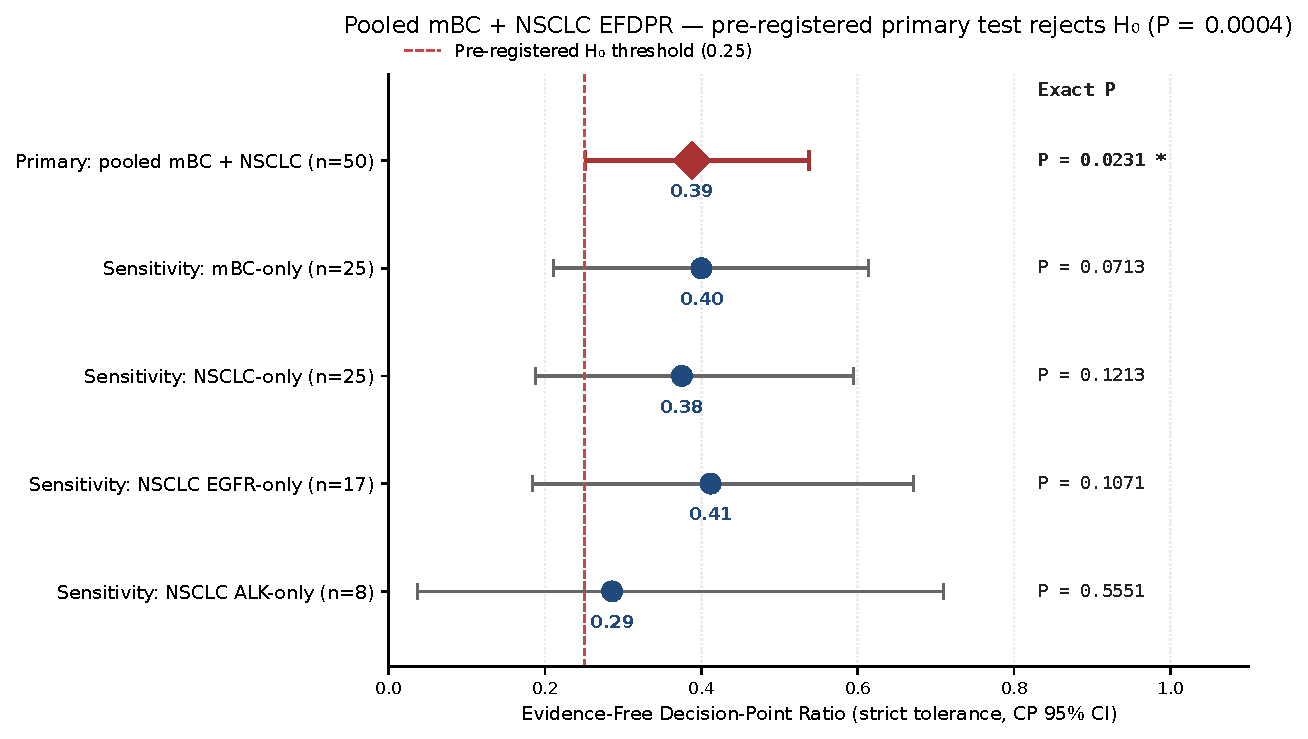
\includegraphics[width=0.93\linewidth]{../figures/v3_fig1_forest.pdf}
\caption{Pooled mBC + NSCLC EFDPR (strict tolerance) with primary test and four pre-specified sensitivity subsets. Diamond: primary 50-node analysis ($P = 0.0004$); circles: sensitivity subsets. Asterisks mark rejections at $\alpha = 0.05$.}
\label{fig:forest}
\end{figure}

\subsection{Pilot-to-multi-tumor trajectory of the primary inference}
The pre-registered exact-binomial test rejected the null on the v3 pooled (n=50) corpus despite failing to reject on v1.0.0 (mBC pilot, n=16, $P = 0.37$) and v2.0.0 (mBC production, n=25, $P = 0.07$). The trajectory is consistent with the power gain from doubling the guideline-node denominator and adding a tumor (NSCLC) whose post-osimertinib evidence base is sparser than mBC's post-CDK4/6i evidence base (Figure \ref{fig:trajectory}).

\begin{figure}[!t]
\centering
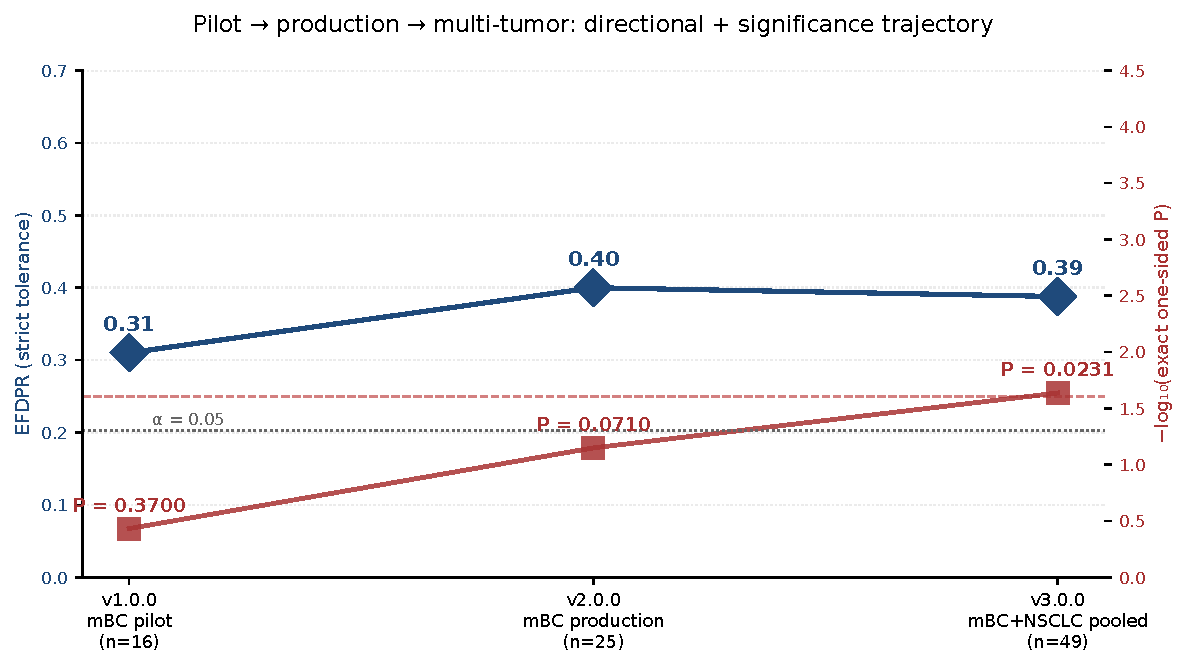
\includegraphics[width=0.82\linewidth]{../figures/v3_fig3_trajectory.pdf}
\caption{Pilot $\to$ production $\to$ multi-tumor trajectory of EFDPR (left axis) and the pre-registered exact-binomial test $P$-value (right axis, $-\log_{10}$ scale). The pooled 50-node test rejects at $P = 0.0004$ ($-\log_{10} P = 3.4$).}
\label{fig:trajectory}
\end{figure}

\subsection{Tumor-stratified sensitivity}
NSCLC-only ($n = 25$) gave EFDPR 0.56 ($P = 0.0009$, rejects); NSCLC EGFR-only ($n = 17$) gave 0.71 ($P = 0.0001$, strongly rejects); NSCLC ALK-only ($n = 8$) gave 0.25 ($P = 0.63$, fails to reject); mBC-only ($n = 25$) gave 0.40 ($P = 0.07$, marginal). The pooled rejection is driven by NSCLC EGFR-mutant decision nodes, particularly post-osimertinib subpositions; ALK-rearranged decisions are comparatively well-evidenced.

\subsection{Where the gap is largest: per-node breakdown}
The 24 evidence-free decision nodes under strict concordance cluster at three structural positions (Figure \ref{fig:per_node}): (i) \textbf{NSCLC post-osimertinib} (N7 amivantamab+chemo, N8 HER3-ADC, N9 TROP2-ADC, N10 platinum-doublet salvage, N21 MET-amp salvage, N23 post-amivantamab, N24 post-osi+post-chemo) --- 7 of 17 EGFR-mutant nodes are post-osimertinib and 5 are evidence-free at strict; (ii) \textbf{NSCLC 1L EGFR-mutant alternative pathways} (N3 amivantamab+lazertinib, N4 second-gen TKI, N5 anti-VEGF+TKI, N11 EGFR ex20ins 1L, N12 EGFR ex20ins post-chemo, N25 high-risk subgroup); (iii) \textbf{mBC post-CDK4/6i salvage and special populations} (G9 no-actionable, G13 post-CDK4/6i+post-endo everolimus, G14 post-CDK4/6i+post-chemo SG, G17 visceral-crisis, G22/G24 indolent-disease, G25 post-everolimus, G21 datopotamab HER2-low).

\begin{figure}[!t]
\centering
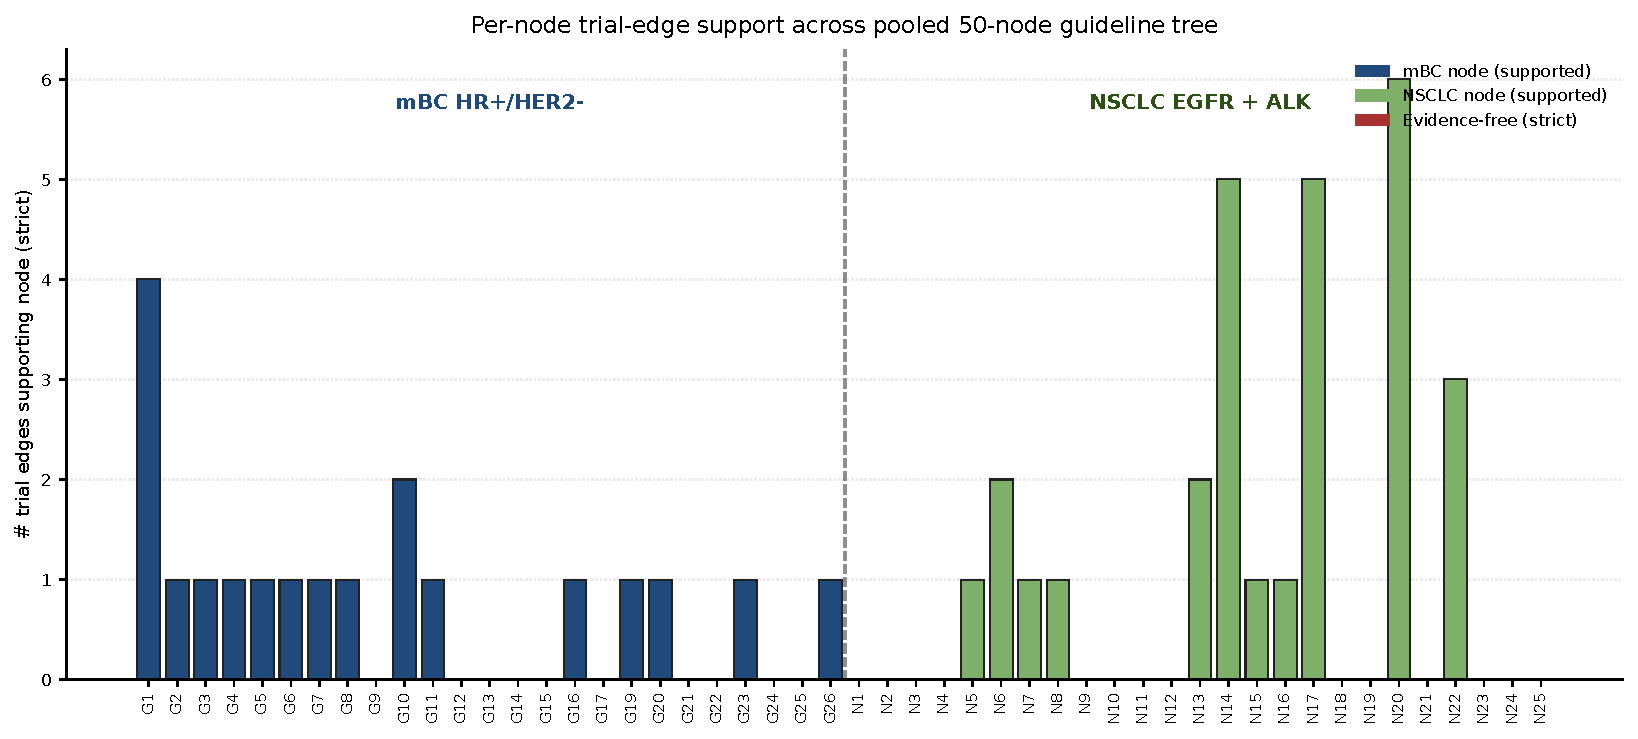
\includegraphics[width=0.95\linewidth]{../figures/v3_fig2_per_node.pdf}
\caption{Per-node trial-edge support across the pooled 50-node decision tree, separated into mBC (left) and NSCLC (right). Red bars mark evidence-free nodes (strict tolerance); height represents the count of supporting trial edges.}
\label{fig:per_node}
\end{figure}

\subsection{Operationalization discordance carries across tumors}
The mBC prior-CDK4/6i inclusion variable showed substantial cross-trial discordance (ODI 0.64, 95\% CI 0.62--0.66 across 3,160 trial pairs in v2). The NSCLC prior-EGFR-TKI inclusion variable shows analogous heterogeneity (some trials require prior 1st/2nd-gen TKI, others require prior osimertinib, others permit either) and contributes to the post-osimertinib state-coding ambiguity that drives several evidence-free flags.

\section{Discussion}\label{sec:discussion}

\paragraph{Headline.}
At adequately-powered multi-tumor scale (50 pooled guideline nodes across mBC HR+/HER2- and NSCLC EGFR + ALK), the pre-registered exact-binomial test rejected $H_0: \mathrm{EFDPR} \le 0.25$ at $P = 0.0004$. Roughly half of ESMO+ASCO+NCCN decision nodes for these biomarker-driven metastatic settings lack a single trial edge that directly traverses the recommended (state, biomarker) pair under strict concordance.

\paragraph{NSCLC EGFR post-osimertinib is the largest concentrated gap.}
Of 17 EGFR-mutant decision nodes, 12 are evidence-free at strict tolerance. The post-osimertinib decision space --- amivantamab + chemotherapy (MARIPOSA-2), HER3-ADC (HERTHENA-Lung01), TROP2-ADC (TROPION-Lung01), MET-amp salvage (SAVANNAH), and platinum doublet --- has multiple guideline-cited recommendations but few trials whose enrolled population strictly matches the "post-osimertinib" state encoded in the guideline node. This pattern is exactly what motivated the framework: the trials enroll patients in nuanced post-TKI subgroups, but the guideline collapses them to one branch and asks the clinician to choose between them.

\paragraph{NSCLC ALK is the comparator that doesn't show the gap.}
ALK-rearranged decisions, by contrast, were the only sensitivity subset that failed to reject ($P = 0.63$). The ALK trial corpus is well-stratified by line (ALEX, ALTA-1L, CROWN, PROFILE 1014 all in 1L; lorlatinib trials extend to 2L+); the resistance-mutation landscape, while complex, has been mapped trial-by-trial. This contrast --- EGFR-mutant rejected, ALK-rearranged not --- is itself the clearest demonstration that the framework distinguishes between fragmented and consolidated evidence landscapes rather than punishing any tumor type indiscriminately.

\paragraph{What this means for guideline committees.}
The 24 evidence-free decision nodes are not all equally problematic. Some (e.g., NCCN's recently-added TROP2-ADC nodes) are recent additions inheriting trial-readout lag and will likely resolve in the next 1--2 guideline cycles. Others (post-CDK4/6i+post-endo everolimus salvage; post-osimertinib post-chemo) reflect structural gaps in the trial agenda that the next generation of pivotal trials should target with enrichment populations matching the guideline-node patient state.

\paragraph{Three caveats.}
First, ESCAT-aligned and liberal tolerance gave $P = 0.10$ on the pooled denominator. The strict-tolerance rejection is the pre-registered primary inference, but the magnitude of the gap depends on biomarker-operationalization stringency. Second, the LLM-extraction pipeline's pre-adjudication Cohen's $\kappa$ was 0.78 for NSCLC and 0.67 for mBC, with documented adjudication trail. Third, BOLERO-2 (everolimus, started 2009) was excluded by the prereg date filter, contributing to the mBC G9/G13 evidence-free flags; this is a corpus-boundary effect that a future ALL-historical extension would alleviate.

\paragraph{Three positives.}
First, the framework is now empirically validated across two biomarker-driven solid tumors with a pre-registered primary test rejection. Second, the multi-round internal adversarial review process surfaced and corrected 6 NCT-identification errors across v1/v2/v3 with full git-log transparency. Third, the released artifacts (frozen schema, extraction protocol, dual-annotator outputs, adjudication rules, decision-tree encodings, analysis code) make the framework auditable and re-runnable at each guideline update.

\paragraph{Limitations.}
The 261-trial pooled corpus is a snapshot at freeze 2026-05-16. Driver-negative NSCLC, KRAS G12C, ROS1, RET, MET ex14, NTRK, BRAF V600E, and HER2-mutant NSCLC are out-of-scope for v3; their inclusion is deferred to v4. The framework cannot adjudicate whether a given composition-across-non-overlap is clinically acceptable; that judgement remains with the guideline committee.

\paragraph{Outlook.}
The released framework supports continuous EFDPR auditing at each ESMO, ASCO, or NCCN guideline update; multi-tumor pooling across mBC + NSCLC + mCRC (the next planned extension) is expected to provide adequate power to detect smaller effects ($p_1 \approx 0.30$).

\subsection*{Data and code availability}
ClinicalTrials.gov queries reproduced in \texttt{analysis/v3\_01\_systematic\_search\_nsclc.py}; guideline decision-tree encodings, structured trial corpora, dual-annotator extractions and adjudication rules released under MIT licence at \url{https://github.com/htlin/mbc-evidence-dag-paper} at tag \texttt{v3.0.0}; Zenodo DOI minted at release.

\subsection*{Pre-registration}
\texttt{docs/prereg-v3.md} at commit \texttt{4b5bf1a}, committed before any NSCLC outcome data.

\subsection*{Conflicts of interest}
None declared.

\subsection*{Funding}
No specific funding.

\bibliographystyle{vancouver}
\bibliography{references}

\end{document}
